\begin{SCfigure*}[][p]
	\centering
	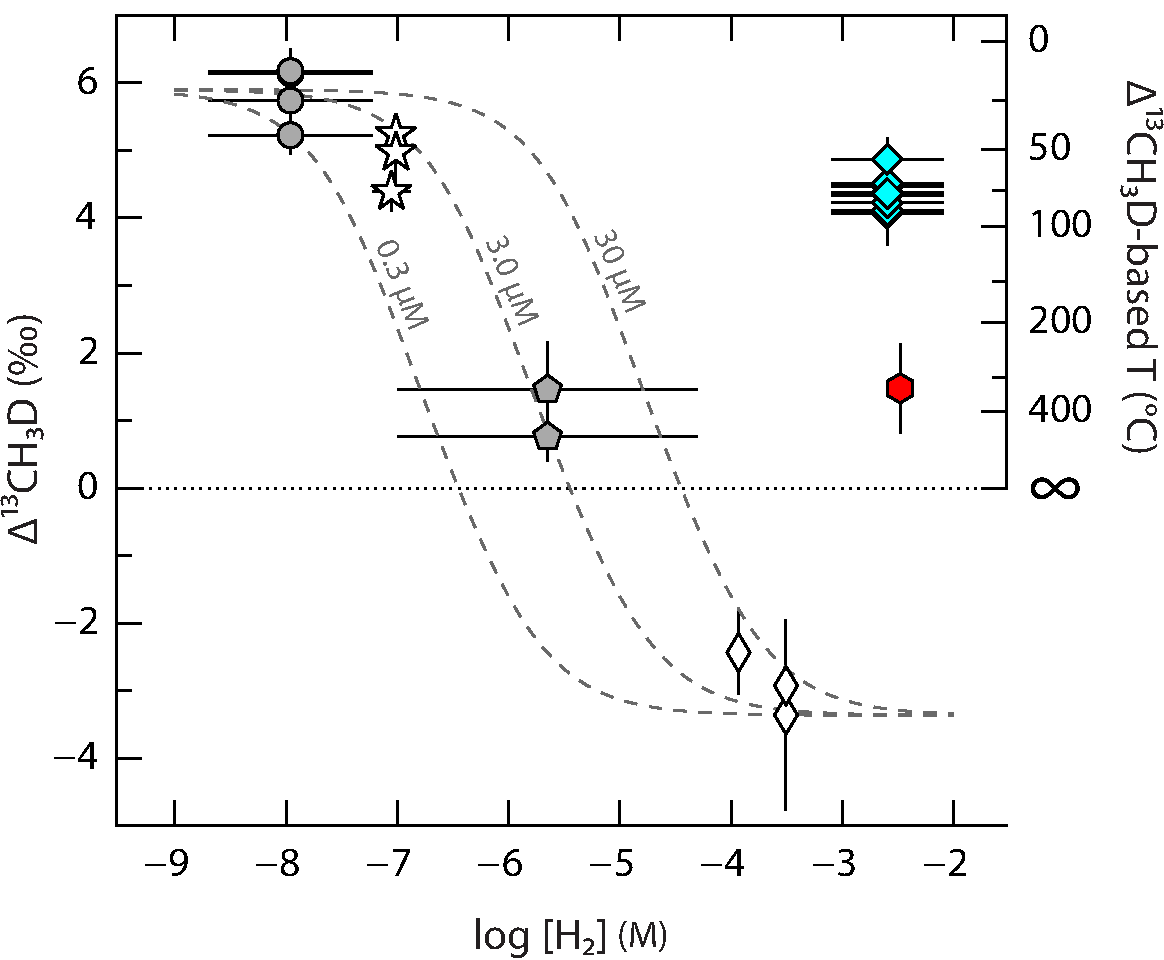
\includegraphics[width=0.5\linewidth]{figures/Fig2.4}
	\caption[Relationships between
	Δ\textsuperscript{13}CH\textsubscript{3}D and H\textsubscript{2}
	concentration for microbial methane]{Relationships between
		Δ\textsuperscript{13}CH\textsubscript{3}D and H\textsubscript{2}
		concentration for microbial methane. Symbols and vertical error bars
	are the same as in \autoref{fig:2:1}. The H\textsubscript{2} data are from \autoref{tab:2:S4}; when a range of {[}H\textsubscript{2}{]} values is given, points are
	plotted at the geometric mean of the maximum and minimum values. Dashed
	lines represent model predictions for microbial methane produced at 20~°C, calculated using \emph{K}\textsubscript{M}'s of 0.3, 3.0, and 30~µM
	H\textsubscript{2}. Data for samples of dominantly non-microbial methane
	from Guaymas Basin and Kidd Creek are plotted for comparison.}
	\label{fig:2:4}
\end{SCfigure*}